\chapter{Proposta de plano de trabalho}

\section{Descrição}

A elaboração da pesquisa aqui proposta pode ser subdividida em algumas seções e atividades a serem distribuídas ao longo de vinte e quatro meses de trabalho e contemplam levantamento de bibliografias e dados, trabalhos de campo, atividades de cunho prático e/ou técnico, além de análise de dados e redação de relatórios e artigos expondo a evolução do trabalho.

A seção de \textbf{levantamento bibliográfico e de dados} consiste em realizar um levantamento das produções bibliográficas, de teorias e métodos geográficos que:

\begin{itemize}
 \item Abordem a técnica e sua influência na configuração do território;
 \item Ressaltem as características da região estudada e as possibilidades e impedimentos dos movimentos sociais locais;
 \item Discutam evidências de impactos ambientais causados pelo agronegócio;
 \item Caracterizem a evolução do uso da técnica e como isso tem impactado a configuração espacial da região de estudo.
 \item Dissertem sobre as possibilidades de organização da sociedade em rede e o papel das redes sociais para a divulgação / organização de movimentos sociais;
\end{itemize}

Já a seção de \textbf{trabalhos práticos} consiste na elaboração de um software utilizando tecnologias livres que tenha a função de um "portal de informações" sobre a região, com notícias, estatísticas e que possibilite o mapeamento colaborativo das áreas afetadas pelo agronegócio, além de outras funcionalidades que surgirão a partir da necessidade de integrantes dos movimentos sociais de combate ao agronegócio da região. Os dados e informações disponíveis no software serão disponibilizados pelos próprios agentes locais da comunidade, afim de alertar, denunciar e/ou divulgar as ações do agronegócio que afetam/destroem os bens naturais e o modo de vida da região. Através do uso desta ferramenta, será possível fortalecer a ação dos movimentos sociais na região através da auto-cartografia dos povos e comunidades tradicionais da amazônia, objetivando maior conhecimento sobre o processo histórico de ocupação dessa região.

Uma das principais motivações para a construção desse software é a possibilidade de integrar às redes sociais as informações e os mapas construídos colaborativamente pela sociedade civil organizada, afim de auxiliar no trabalho de movimentos sociais que focam suas ações na evolução da situação na região em relação às ações do agronegócio. Com o uso da técnica e do poder informacional, acreditamos ser possível facilitar o exercício do contrapoder pelos movimentos sociais, agora em rede.

Este software será construído com base em metodologias ágeis\footnote{São metodologias de desenvolvimento de software baseadas em processos iterativos e incrementais de planejamento, execução, validação e reflexões sobre as decisões tomadas. Essas metodologias, como o SCRUM e a programação extrema, visam o contínuo incremento de valor ao produto, afim de maximizar a qualidade e a real utilidade do software.} de desenvolvimento, computação em nuvem\footnote{De forma simplória, a computação em nuvem é baseada na utilização de recursos de infra-estrutura e/ou serviços disponíveis na própria internet, eliminando a necessidade de criar uma estrutura física de servidores para publicar uma aplicação na internet.} e tecnologias livres\footnote{Tecnologias onde existe liberdade para utilizar, estudar, modificar e redistribuir a tecnologia original.}, sendo disponibilizado em ambiente de código-aberto\footnote{O código-fonte gerado para a construção do software estará disponível ao público na internet.}, para livre utilização pela comunidade.

Já para a seção de \textbf{trabalhos técnicos}, propõe-se a confecção de croquis e mapas sobre a evolução dos impactos sócio-ambientais na área de estudo, baseado nas informações obtidas através do software elaborado na seção de trabalhos práticos e nos trabalhos de campo realizados.

A \textbf{análise dos dados}, ocorrerá de forma constante, visando o direcionamento e a elaboração do trabalho da pesquisa. 

Para divulgação do resultado da pesquisa, pretende-se elaborar um ou mais artigos para submissão e publicação em periódicos especializados de geografia e/ou em computação, relatando algumas das considerações acerca da pesquisa, além da elaboração da dissertação de mestrado e apresentação dos resultados da pesquisa em eventos científicos com a temática da geografia, e do processo de construção do software em eventos de engenharia e desenvolvimento de software.

\section{Cronograma}

O cronograma prevê 24 meses de atividades, dispostas conforme o quadro abaixo:

\begin{figure}[htb]
\begin{center}
    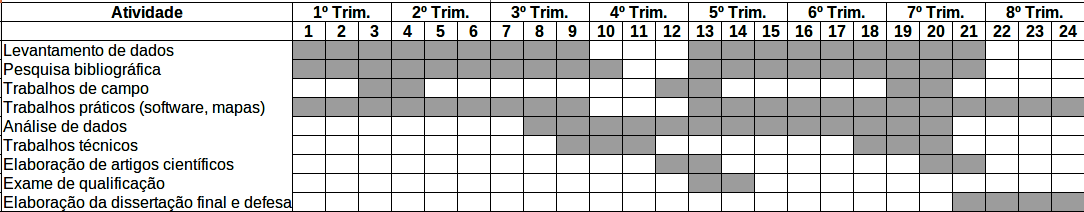
\includegraphics[scale=0.4]{crono.png}
\end{center}
\end{figure}


\begin{table}[htb]

\end{table}

\begin{quadro}[htb]
\caption{\label{quadro_modelo}Caption do quadro}
Este é o conteúdo do quadro.
\ABNTEXfontereduzida
\caption[Cronograma]{Cronograma de atividades}
\label{tab-nivinv}
\begin{tabular}{p{2.6cm}|p{6.0cm}|p{2.25cm}|p{3.40cm}}
  \hline
\\
   \textbf{Nível de Investigação} & \textbf{Insumos}  & \textbf{Sistemas de Investigação}  & \textbf{Produtos}  \\
    \hline
    Meta-nível & Filosofia\index{filosofia} da Ciência  & Epistemologia &
    Paradigma  \\
    \hline
    Nível do objeto & Paradigmas do metanível e evidências do nível inferior &
    Ciência  & Teorias e modelos \\
    \hline
    Nível inferior & Modelos e métodos do nível do objeto e problemas do nível inferior & Prática & Solução de problemas  \\
    \hline
\end{tabular}
\legend{Fonte: \citeonline{van86}}
\end{quadro}
